\chapter{Ergänzende Abbildungen}

\begin{figure}[H]
    \label{fig:ContourComplexFun}
    \centering
    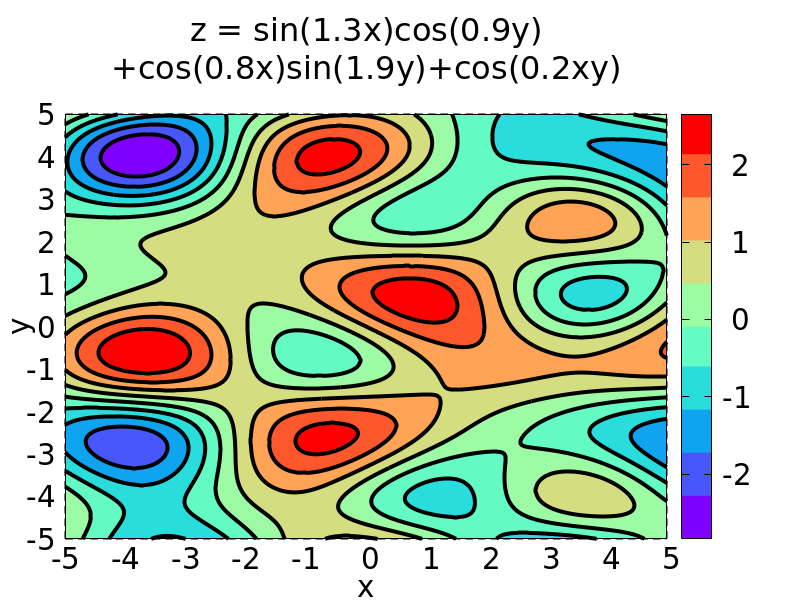
\includegraphics[width=0.95\textwidth]{./gnuplot/example-contour-field-complex}
    \caption{Konturlinien mit farbiger Hervorhebung für eine Funktion. Jede Farbe entspricht einem Funktionswert, wie er in der Legende rechts zu sehen ist.}
\end{figure}

\begin{figure}[H]
    \label{fig:UniLogScale}
    \centering
    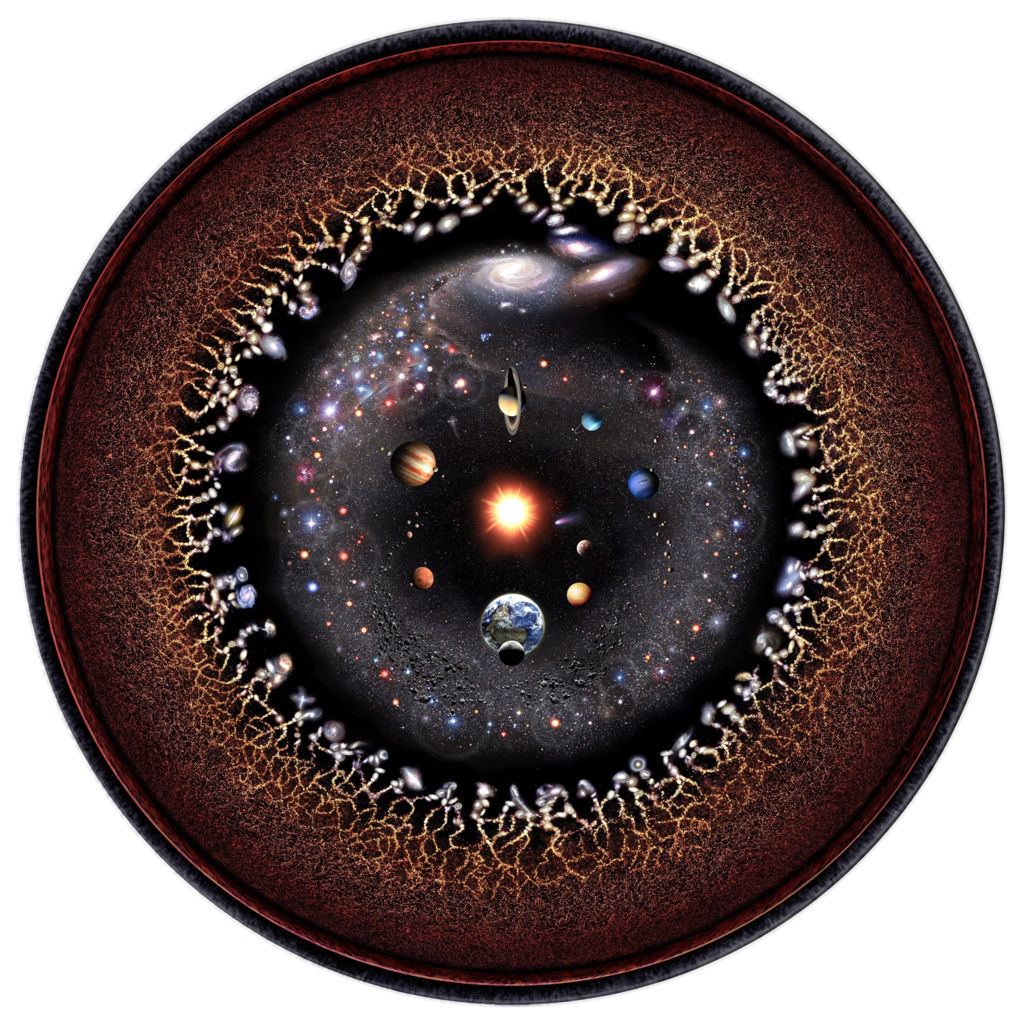
\includegraphics[width=0.95\textwidth]{./img/universe-log-scale}
    \caption{Künstlerische Darstellung des beobachtbaren Universums in logarithmischer Skalierung und Zentrierung auf das Sonnensystem. Abgebildet sind die inneren und äußeren Planeten des Sonnensystems, der Kuipergürtel, die Oortsche Wolke, Alpha Centauri, Perseusarm, die Milchstraße, der Andromedanebel, Nachbargalaxien, das Kosmische Netz, die Kosmische Hintergrundstrahlung und der Plasmazustand kurz nach dem Urknall. Quelle: \href{https://commons.wikimedia.org/wiki/User:Unmismoobjetivo}{Pablo Carlos Budassi}, \href{https://commons.wikimedia.org/wiki/File:Observable_universe_logarithmic_illustration.png}{wikimedia}}
\end{figure}
